\renewcommand*{\arraystretch}{1.1}

\noindent\begin{tabularx}{17cm}{|p{1.95cm}|X|}
	\hline
	workload    & BI \\ \hline
%
	query       & 12 \\ \hline
%
	title       & Trending Posts \\ \hline
%
    pattern     & \hfill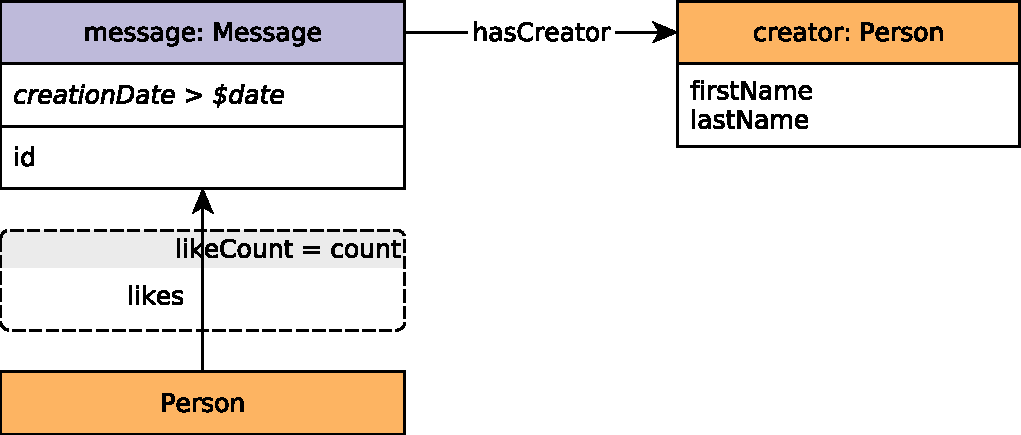
\includegraphics[scale=\patternscale,margin=0cm .2cm]{patterns/bi-read-12}\hfill\vadjust{} \\ \hline
%
	description & Find all Messages created after a given date, that received more than a
given number of likes.
 \\ \hline
%
	
%
	parameters  &
	\vspace{1.1ex}{\begin{tabularx}{14.2cm}{|c|M|m{2cm}|Y|} \hline
	\cellcolor{parameter} \color{white} $\mathsf{1}$ & \varname{creationDate} & \cellcolor{gray!20} \vartype{Date} &  \\ \hline
	\cellcolor{parameter} \color{white} $\mathsf{2}$ & \varname{likeThreshold} & \cellcolor{gray!20} \vartype{32-bit Integer} &  \\ \hline
	\end{tabularx}}\vspace{1.1ex} \\ \hline
%
	
	result      &
	\vspace{1.1ex}{\begin{tabularx}{14.2cm}{|c|M|m{2cm}|c|Y|} \hline
	\cellcolor{result} \color{white} $\mathsf{1}$ & \varname{message.id} & \cellcolor{gray!20} \vartype{64-bit Integer} &
	    \texttt{R} &
	     \\ \hline
	\cellcolor{result} \color{white} $\mathsf{2}$ & \varname{message.creationDate} & \cellcolor{gray!20} \vartype{DateTime} &
	    \texttt{R} &
	     \\ \hline
	\cellcolor{result} \color{white} $\mathsf{3}$ & \varname{creator.firstName} & \cellcolor{gray!20} \vartype{String} &
	    \texttt{R} &
	    The first name of the post's creator \\ \hline
	\cellcolor{result} \color{white} $\mathsf{4}$ & \varname{creator.lastName} & \cellcolor{gray!20} \vartype{String} &
	    \texttt{R} &
	    The last name of the post's creator \\ \hline
	\cellcolor{result} \color{white} $\mathsf{5}$ & \varname{likeCount} & \cellcolor{gray!20} \vartype{32-bit Integer} &
	    \texttt{A} &
	    The number of Likes the Post received \\ \hline
	\end{tabularx}}\vspace{1.1ex} \\ \hline
	
%
	sort        &
	\vspace{1.1ex}{\begin{tabular}{|c|l|c|} \hline
	\cellcolor{sort} \color{white} $\mathsf{1}$ & \varname{likeCount} & \cellcolor{gray!20} $\desc$ \\ \hline
	\cellcolor{sort} \color{white} $\mathsf{2}$ & \varname{message.id} & \cellcolor{gray!20} $\asc$ \\ \hline
	\end{tabular}}\vspace{1.1ex} \\ \hline
	%
	limit       & 100 \\ \hline
	%
	choke points &
	\multicolumn{1}{>{\raggedright}l|}{
	  \chokepoint{1.2}, 
	  \chokepoint{2.2}, 
	  \chokepoint{3.1}, 
	  \chokepoint{6.1}
	  } \\ \hline
	%
\end{tabularx}
\vspace{2ex}